%
%% 2019 07 04 Ph. G. Freimann
%%

\section{Lineare Gleichungen\TALS{ I}}\index{Gleichungen!lineare}\index{Lineare Gleichung}\label{gleichungen_lineare}
\sectuntertitel{... weil keine zwei Dinge gleicher sein
  können.\footnote{\textit{Robert Recorde} (1557; \textit{Der
      Wetzstein des Wissens}) über das
    Gleichheitszeichen\index{Gleichheitszeichen} als zwei Parallele:
    «... weil keine zwei Dinge gleicher sein können.»}}

%%\TALSTadBFWA{81}{2.2}
%%%%%%%%%%%%%%%%%%%%%%%%%%%%%%%%%%%%%%%%%%%%%%%%%%%%%%%%%%%%%%%%%%%%%%%%%%%%%%%%%
\subsection*{Lernziele}

\begin{itemize}
\item Lineare Gleichungen
\item Äquivalenzumformung / Lösungsmenge
\item Grundform (GF) linearer Gleichungen
\item Textaufgaben, die zu Gleichungen\index{Textgleichungen}\TALS{
  (ev. mit Parametern)} führen.
\TALS{\item Einsatz des Taschenrechners}
\end{itemize}

\TadBMTA{115}{8}

\subsection{Typen von Gleichungen}
\begin{bbwFillInTabular}{ll}\hline
  Bestimmungsgleichung & $5x + 6  =  8x-3$            \\\hline
  Identitätsgleichung  & $(a+b)^2 =  a^2 + 2ab + b^2$  \\\hline
  Definitionsgleichung & $\pi     := \frac{U}{2r}$    \\\hline
  \end{bbwFillInTabular} 

\newpage

\TRAINER{\GESO{Bem. «Lineare Gleichungen erst mal ohne ohne Parameter»}}
\noTRAINER{\vspace{10mm}}


\begin{beispiel}{Einstiegsbeispiel}{}

$$\sqrt{2}(x+5) = 3x + \sqrt{7} - \frac{x}4$$

  Die \textit{harte} Tour:
  
  \TNT{13.2}{ 1. Ausmultiplizieren

    \begin{tabular}{ll}

      $x\sqrt{2} + 5\sqrt{2}            = 3x + \sqrt{7} -\frac14x$ &  $| + \frac14x$\\

      $x\sqrt{2} + 5\sqrt{2} + \frac14x =  3x + \sqrt{7}$          &  $| - 3x$\\

      $x\sqrt{2} + 5\sqrt{2} + \frac14x -3x =   \sqrt{7}$          &  $| -5\sqrt{2}$\\

      $x\sqrt{2} + \frac14x -3x =   \sqrt{7} - 5\sqrt{2}$          & $| x\text{ ausklammern}$\\

      $x (\sqrt{2} + \frac14 -3) =   \sqrt{7} - 5\sqrt{2}$          &      $| x\text{ durch Klammer teilen}$\\

      $x = \frac{  \sqrt{7} - 5\sqrt{2}}{\sqrt{2} + \frac14 -3}$          &      $| x\text{ durch Klammer teilen}$\\

      $x \approx   3.31289$    &    \\

    \end{tabular}

Allenfalls Probe mit TR:
\GESO{\tiprobutton{sto}\tiprobutton{xyzabcd}}
\TALS{$x:= \frac{  \sqrt{7} - 5\sqrt{2}}{\sqrt{2} + \frac14 -3}$},
dann $x$ links und rechts einsetzen: Term wird je $ 11.7562$.
\vspace{55mm}
}%% END TNT

\end{beispiel}


\begin{definition}{Lineare Gleichung}{definition_lineare_gleichung}
  Salopp: Bei einer \textbf{linearen Gleichung} kommt die Gesuchte in der
  1. Potenz vor; \zB $x (= x^1)$.
\end{definition}
\newpage

\begin{rezept}{Lineare Gleichung auflösen}{}
  \begin{enumerate}
    \item In einzelne Summanden verwandeln (ausmultiplizieren)
  \item sortieren: Alle Summanden, welche den Faktor $x$ enthalten, auf eine Seite bringen (alle «nicht $x$» auf die andere Seite)
  \item $x$ ausklammern
  \item durch die Klammer teilen
    \end{enumerate} 
  \end{rezept}
\newpage

\subsection{Äquivalenzumformungen}\index{Aquivalenzumformungene@Äquivalenzumformungen}
Äqui... = Gleich...; ...valenz = ...wertig

\TadBMTA{111ff}{7.2}
%%\TALS{S. \cite{frommenwiler17alg} Seite 79 (Äquivalenz von Aussageformen)}
%%\TALS{S. \cite{frommenwiler17alg} Seite 80 (Liste der Äquivalenzumformungen)}
%%\GESO{S. \cite{marthaler21alg} Seite 111 (Liste der Äquivalenzumformungen)}


\textbf{{\color{ForestGreen}Äquivalenzumformungen sind}\TRAINER{\footnote{Mit $|$
      bezeichnen wir den Umformungsstrich}}}

\begin{tabular}{lp{6cm}p{8cm}}\hline\\%%
Umformung   & Beschreibung  & Beispiel \\\hline
$| $ TU      & Termumformung & {\raggedright Beispiel: Links des Gleichheitszeichens $a$ ausklammern; gilt , sofern sich die Definitionsmenge des Terms nicht ändert!}\\
$| $ $+ T(x)$  & Term beidseitig addieren. & $| \noTRAINER{........}\TRAINER{\color{ForestGreen}+4}$, $| \noTRAINER{........}\TRAINER{\color{ForestGreen}+\sqrt{x}}$, $| \noTRAINER{.......}\TRAINER{\color{ForestGreen}+8\cdot{}x^2}$\\
$| $ $- T(x)$  & Term beidseitig subtrahieren. & $| \noTRAINER{........}\TRAINER{\color{ForestGreen}-6}$, $|\noTRAINER{........}\TRAINER{\color{ForestGreen}-x^3}$, $|\noTRAINER{.......}\TRAINER{\color{ForestGreen} -\frac1{x}}$\\
$| $ $\cdot{} T$  & Mit von Null verschiedenem Term $T$ multiplizieren. & $| \noTRAINER{......}\TRAINER{\color{ForestGreen}\cdot{} 3}$, $|\noTRAINER{..........}\TRAINER{\color{ForestGreen}\cdot{}(2+\sqrt{x})}$, $|\noTRAINER{.......}\TRAINER{\color{ForestGreen}\cdot{}a^2; a\ne 0}$\\
$| $ $: T$  & Durch von Null verschiedenem Term $T$ dividieren. & $| \noTRAINER{.......}\TRAINER{\color{ForestGreen}: 6}$, $|\noTRAINER{.......}\TRAINER{\color{ForestGreen}: \frac{\pi}6}$, $|\noTRAINER{..............}\TRAINER{\color{ForestGreen}:\sqrt{b}; b> 0}$\\
\end{tabular}

\textbf{\color{red} {keine} Äquivalenzumformungen sind}

\begin{tabular}{lp{6cm}>{\raggedright}p{4cm}p{4cm}}\hline\\
Umformung  & Beschreibung &Lösungen können... & Beispiel\\\hline\\
%%$| $ TU & Termumformung & ... ändern & {| \color{red} TU $(x+1)$ kürzen}\\
$| $ potenzieren  & Beide Seiten potenzieren & \LoesungsRaum{...hinzukommen.}&$| \noTRAINER{......}\TRAINER{\color{red}\Box{}^6}$\\
$| $ radizieren & Auf beiden Seiten die Wurzel ziehen& \LoesungsRaum{...verschwinden.}&$| \noTRAINER{.......}\TRAINER{\color{red}\sqrt[4]{\,}}$\\
$| $ $\cdot{}T(x)$  & mit der Unbekannten multiplizieren & \LoesungsRaum{...hinzukommen.}&$| \noTRAINER{..............}\TRAINER{\color{red}\cdot{}(2-\sqrt{x})}$, $| \noTRAINER{.......}\TRAINER{\color{red}\cdot{}3x^2}$\\
$| $ $:T(x)$  & durch Unbekannte dividieren & \LoesungsRaum{... verschwinden.}&$|
\noTRAINER{..............}\TRAINER{\color{red}:(x-8)}$, $| \noTRAINER{.......}\TRAINER{\color{red}:\sqrt{x}}$\\

\end{tabular}
\newpage

\subsubsection{Finde Äquivalenzumformungen (optional)}
Der folgende Lösungsweg ist definitiv falsch. Irgendwo ist eine Umformung vorgenommen worden, die nicht gültig ist.
Schreiben Sie bei jeder Umformung hin, um welche der oben angegebenen gültigen Äquivalenzumformung es sich handelt. Finden Sie den Fehler:

Im folgenden seien $\pi$ und $a$ als die Kreiszahl $3.14159...$
definiert. Es gilt also $\pi = a$.


\begin{tabular}{lr@{$=$}lp{7cm}}
                  & $a$              & $\pi$               & nach Voraussetzung       \\
$\Longrightarrow$ & $a\cdot a$       & $a\cdot\pi$         & wegen .........................     \\ 
$\Longrightarrow$ & $a^2$            & $a\pi$              & ................................... \\ 
$\Longrightarrow$ & $a^2 + a^2$      & $a\pi + a^2$         & ................................... \\
$\Longrightarrow$ & $2a^2$           & $a\pi + a^2$         & ................................... \\ 
$\Longrightarrow$ & $2a^2-2a\pi$     & $a\pi + a^2 -2a\pi$  & ................................... \\ 
$\Longrightarrow$ & $2a^2-2a\pi$     & $\,\,\,\,\,\,\,\,\,\,\,\,\,\,  a^2 -a\pi$  & ................................... \\ 
$\Longrightarrow$ & $2a^2-2a\pi$     & $a\cdot(a-\pi)$     & ................................... \\ 
$\Longrightarrow$ & $2a\cdot(a-\pi)$ & $a\cdot(a-\pi)$     & ................................... \\ 
$\Longrightarrow$ & $\frac{2a\cdot(a-\pi)}{a-\pi}$ & $\frac{a\cdot(a-\pi)}{a-\pi}$     & \noTRAINER{...................................} \TRAINER{hier wurde durch 0 dividiert, denn $a=\pi$!}\\ 
$\Longrightarrow$ & $2a$             & $\frac{a\cdot(a-\pi)}{a-\pi}$     & \noTRAINER{...................................}\TRAINER{Definitionsbereich durch Termumformung links verändert} \\ 
$\Longrightarrow$ & $2a$             & $a$                 & \noTRAINER{...................................}\TRAINER{Definitionsbereich durch Termumformung rechts verändert} \\ 
$\Longrightarrow$ & $2$              & $1$                 & ........................ \\ 
\end{tabular}

\subsection*{Aufgaben}
\AadBMTA{127ff}{2. a) g) f)}

\newpage

\subsection{Spezielle lineare Gleichungen}
\textbf{Typ A}\\

$$1+4x+2 = 5x - (x-3)$$
\TNT{7.2}{Alle Zahlen $x$ lösen die Gleichung!\vspace{14mm}}%% END TNT

\textbf{Typ B}\\

$$3x+8 = 5x-2(x-3)$$
\TNTeop{Keine Zahl $x$ löst die Gleichung!\vspace{14mm}}%% END TNT


\subsection{Lösungsmenge}\index{Lösungsmenge}
  Die Zahlmenge, der gefundenen Lösungen einer Gleichung, nennen wir
  die Lösungsmenge und bezeichnen diese mit $\LoesungsMenge{}$. Falls die gefundene
  Variable $x$ \zB{} \textbf{den Wert $4$} hat, dann schreiben wir:
  $$\LoesungsRaumLang{\lx=\{4\}}$$

  Wenn eine Gleichung \textbf{mehrere Lösungen} hat (\zB $x=7$ und $x=-3$), so
  schreiben wir die Lösungsmenge in aufsteigender Form:
  $$\LoesungsRaumLang{\lx=\{-3; 7\}}$$

  Falls \textbf{alle Zahlen} $x$ die Gleichung \textbf{lösen} (Typ A), so schreiben wir:
  $$\LoesungsRaumLang{\lx=\mathbb{R}}$$


  Eine Gleichung \textbf{ohne Lösung} (Typ B) hat die leere Menge als Lösungsmenge und
  wir schreiben:
  $$\LoesungsRaumLang{\lx=\{\}}$$

  

\subsection*{Aufgaben}
\AadBMTA{127ff}{3.  a) h), 4. f) und 6. a) d) e) f)}
%%\TALSAadBMTA{81}{223. a) b) e) 225. a) d) e) f) 227.a) b) c) 225. a) d) e) f) 229. a) 230. a) 231. d) 232. b)}

\olatLinkGESOKompendium{2.1.1.}{10}{1. bis 6.}

\newpage

\index{Lineare Gleichung!Grundform}\index{Grundform!lineare Gleichung}

\subsection{Grundform}
\begin{definition}{Grundform}{}\index{Grundform!lineare Gleichung}\index{Lineare Gleichung!Grundform}
  \textbf{Grundform}\index{Grundform!lineare Gleichung}:\\

  Eine Gleichung, die äquivalent zu folgender Grundform ist, heißt
  \textbf{lineare Gleichung}:\\
  $$ax+b=0 \text{ mit } a,b\in\mathbb{R}, a\ne 0$$
  
  \end{definition}

\begin{gesetz}{Lösungsformel}{}
 Lösung der linearen Gleichung in der Grundform

 $$ax+b=0$$
 \TNT{2}{$$ax=-b$$\vspace{10mm}}
  $$x = \frac{-b}a$$
  
\end{gesetz}


\subsubsection{Beispiele zur Grundform (optional)}


\begin{beispiel}{Grundform}{beispiel_lineare_gleichung_grundform}
  Bringen Sie die folgende lineare Gleichung auf die Grundform:
  $$2x-10 = -3x\TRAINER{\,\,\,| +3x}$$

  Grundform: $\LoesungsRaum{5x-10} = 0$

  $a = \LoesungsRaum{5}$

  $b = \LoesungsRaum{-10}$

  und somit

  \LARGE{$x=\frac{-(\noTRAINER{\,\,\,\,\,\,}\TRAINER{-10})}{\noTRAINER{\,\,\,\,\,\,\,}\TRAINER{5}}
    = \LoesungsRaum{2}$}

\end{beispiel}


\begin{beispiel}{Lineare Gleichung}{beispiel_lineare_gleichung_3x7}
  Die Gleichung $3x=-7$ ist äquivalent zur Grundform $3x+7=0$ und somit ist die Lösung $\LoesungsRaum{\frac{-7}{3}}$
  \end{beispiel}

\begin{beispiel}{Lineare Gleichung}{beispiel_lineare_gleichung_5x8}
  Die Gleichung $-5x=8$ ist äquivalent zur Grundform $-5x-8=0$ und somit ist die Lösung $\LoesungsRaum{\lx=\frac{8}{-5}}$
\end{beispiel}
\newpage


\newpage
\TALS{%%
%% 2019 11 14 Ph. G. Freimann
%%

\subsection{Gleichungen mit CAS lösen (optional)}\index{CAS@Computer Algebra System}\index{Computer Algebra System@CAS}
Damit weniger Fehler geschehen, aber auch, um schneller an Resultate zu gelangen werden in der Praxis Gleichungen fast ausschließlich mit einem Computer-Algebra-System (CAS) gelöst.
Wir wählen eine einfache Gleichung, damit wir a) nicht viel tippen müssen und b) das Resultat auch sofort überprüfen können. Gegeben ist also die folgende Gleichung:

$$3x+1=2x$$

Typischerweise bieten sich die folgenden drei Lösungswege an\footnote{Die drei Verfahren wurden mit dem Rechner ``TI-nspire II-CX CAS'' getestet.}:
\begin{itemize}
\item solve($3x+1=2x$, $x$)
\item $\text{gl1} := 3x+1=2x$\\
  solve($\text{gl1}$, $x$)
  
\item $\text{term1} := 3x+1$\\
  $\text{term2} := 2x$\\
  solve($\text{term1}=\text{term2}$, $x$)\\
  Diese letzte Variante hat den Vorteil, dass wir die Terme leicht als Funktionen in $x$ auffassen können und diese im Graph-Modus sofort anzeigen können:
  \begin{enumerate}
    \item Neue «Page» (1.2) erstellen (+page) als Graph. 
    \item Tippe $f1(x)=\text{term1}$
    \item Tippe \fbox{CTRL} \fbox{G} (oder mehrmals die \fbox{TAB}-Taste), um die Eingabezeile wieder zu aktivieren.
      \item $f2(x)=\text{term2}$
  \end{enumerate}

\bbwCenterGraphic{6cm}{tals/gl1/img/nspire_zwei_gleichungen.png}
%  \begin{center}
%   \raisebox{-1cm}{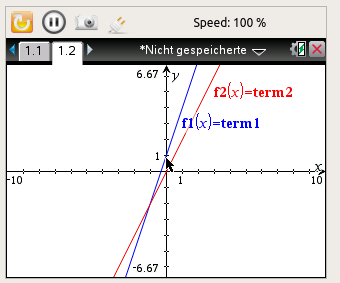
\includegraphics[width=6cm]{img/nspire_zwei_gleichungen.png}}
%  \end{center}
  Der Schnittpunkt der beiden Geraden zeigt die Variable $x$ (hier $-1$) und den Wert der beiden Terme (links bzw. rechts) des Gleichheitszeichens als Variable $y$ (hier $-2$) an.

\end{itemize}

\newpage
\newpage}
\TALS{%%
%% 2020 graphische Interpretation linearer Gleichungen (TALS nSpire)
%%


\newpage
\subsection{Graphische Interpretation}
Graphische Interpretation der Grundform:

In der Form
$$ax+b=0$$
ist $a$ die Steigung\footnote{Steigung: Eine Einheit nach rechts: Um wie viele Einheiten steigt die Gerade an?} der Geraden und $b$ der Abschnitt\index{Achsenabschnitt} auf der $y$-Achse\footnote{$y$-Achsenabschnitt: Wo schneidet die Gerade die $y$-Achse.}:

\bbwCenterGraphic{6cm}{allg/gleichungen/img/LineareGleichungsfunktion.png}
%  \begin{center}
%   \raisebox{-1cm}{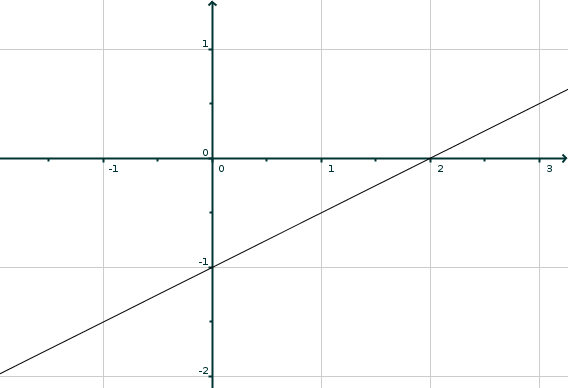
\includegraphics[width=6cm]{img/LineareGleichungsfunktion.png}}
%  \end{center}

  \paragraph{Charakteristische Punkte}
  Die charakteristischen Punkte (spezielle Punkte) der linearen
  Funktion in Grundform sind

  \begin{itemize}
  \item $b$ = $y$-Achsenabschnitt: Wo schneidet die Gerade die $y$-Achse?
  \item $a$ = Steigung der Geraden pro eine Einheit nach rechts (in $x$-Richtung)
  \item $\frac{-b}{a}$ = Lösung der Gleichung $ax+b=0$. Dies ist der $x$-Achsenabschnitt.
  \end{itemize}

}
  
\GESO{%%
%% (C) 2022 ph. freimann @ bbw.ch
%%

\subsection{Gleichungen mit dem Solver lösen}\index{Solver}\index{num-Solv}

«Die \textit{sanfte} Tour»

Lineare Gleichungen ohne Parameter können mit dem Taschenrechner mit dem numerischen
\textit{Solver} (num-solve) gelöst werden.

  Hierzu dient die Taste \tiprobutton{sin_num-solv}.

  Tippen Sie also \tiprobutton{2nd}, dann \tiprobutton{sin} und geben
  Sie die folgende lineare Gleichung ein:

$$\sqrt{2}(x+5) = 3x + \sqrt{7} - \frac{x}4$$

  Alle Optionen sind standardmäßig auf die Suche nach $x$
  eingestellt. Sie müssen also nur \textbf{sechs mal} \tiprobutton{enter}
  drücken um auf $x\approx \LoesungsRaum{3.31289}$ zu kommen!

  \begin{bemerkung}{Limitation}{}\index{Taschenrechner!Limitation}

    Berechnen Sie mit dem numerischen Solver
    \tiprobutton{sin_num-solv} das $x$ in der folgenden
    Bestimmungsgleichung:

    $$x+1=x+2$$
    
    \TNT{4}{Der \textbf{num-Solver} versucht das Resultat anzunähern
      und erhält

      $$x \approx 1.845 \cdot{} 10^{12}$$

      
    }% end TNT

    \vspace{10mm}
    
    \TNT{2}{\textbf{Resultate des Taschenrechners immern nachkontrollieren!}}
    
  \end{bemerkung}
\newpage
  
\subsection*{Aufgaben}
Lösen Sie mit dem Taschenrechner (num-solv):

\GESO{\olatLinkArbeitsblatt{Lineare Gleichungen}{https://olat.bms-w.ch/auth/RepositoryEntry/6029794/CourseNode/110662976644490}{Aufgabe 1. b) c) d) f), 2. a) b)}}

\newpage
}

\newpage
